% !TEX root =  master.tex
\chapter{Literaturverzeichnis}

	\textbf{[B1] Engebretson, P. (2013).
	The basics of hacking and penetration testing: ethical hacking and penetration testing made easy. Elsevier.} \\
	\url{http://dspace.fudutsinma.edu.ng/xmlui/bitstream/handle/123456789/845/ebooksclub.org__The_Basics_of_Hacking_and_Penetration_Testing__Ethical_Hacking_and_Penetration_Testing_Made_Easy.pdf?sequence=1}
	
	
	\textbf{[B2] Yaworski, P. (2018): Web Hacking 101. No Starch Press.} \\
	\url{https://digtvbg.com/files/books-for-hacking/Web%20Hacking%20101%20-%20How%20to%20Make%20Money%20Hacking%20Ethically%20by%20Peter%20Yaworski.pdf}
	
	\textbf{[B3] Mastering Defensive Security by Cesar Bravo, Darren Kitchen.} \\
	\url{https://learning.oreilly.com/library/view/mastering-defensive-security/9781800208162/B16290_FM_Final_JC_ePub.xhtml}
	
	\textbf{[B4] Penetration Testing - A Hands-On Introduction to Hacking}
	


\section{Quellenerzeichnis}

	\textbf{[1] Siemens Indusrty Software Inc.} \\
	Intelligentere Entscheidungen, bessere Produkte durch umfassendes PLM \\
	\url{https://www.plm.automation.siemens.com/de_de/Images/tc_overview_tcm73%-62348.pdf}
	
	\textbf{[2] Cost of data breach 2022} \\
	\url{https://www.ibm.com/reports/data-breach}
	
	\textbf{[3] Patrick Engebretson "The Basics of hacking
		and penetration testing"} \\
	\url{http://dspace.fudutsinma.edu.ng/xmlui/bitstream/handle/123456789/845/ebooksclub.org__The_Basics_of_Hacking_and_Penetration_Testing__Ethical_Hacking_and_Penetration_Testing_Made_Easy.pdf?sequence=1}
	
	\textbf{[4] Deep Learning und Pentesting} \\
	\url{http://repository.kpi.kharkov.ua/handle/KhPI-Press/54956}
	
	\textbf{[5] CHIEM TRIEU PHONG, A Study of Penetration Testing Tools
		and Approaches} \\
	\url{https://openrepository.aut.ac.nz/bitstream/handle/10292/7801/ChiemTP.pdf?sequence=3&isAllowed=y}
	
	\textbf{[6] A Study on Penetration Testing Process and Tools } \\
	\url{https://ieeexplore.ieee.org/stamp/stamp.jsp?arnumber=8378035&casa_token=XNKWbXqAGogAAAAA:zi_TswzVWQeWmdEiCATwmOxCQ_L8-exnSsgQQQBM3ahGCG2iCg5ciNeyWkrBJxe6sdI7n4ycT11MBEY&tag=1}
	
	\textbf{[7] Shah, M. P. (2020). Comparative analysis of the automated penetration testing tools (Doctoral dissertation, Dublin, National College of Ireland).} \\
	\url{https://norma.ncirl.ie/4165/1/mandarprashantshah.pdf}
	
	\textbf{[8] Penetration Testing in a Web
		Application Environment} \\
	\url{http://www.diva-portal.org/smash/get/diva2:356502/fulltext01.pdf}
	
	Das hier später noch Aufräumen und Citavi oder so verwedent
	
	weitere Quellen
	
	\url{https://sectooladdict.blogspot.com/}
	
	\url{https://owasp.org/www-community/Vulnerability_Scanning_Tools}
	
\section{Bildverzeichnis}


\begin{figure}[H]
	\centering 
	\frame{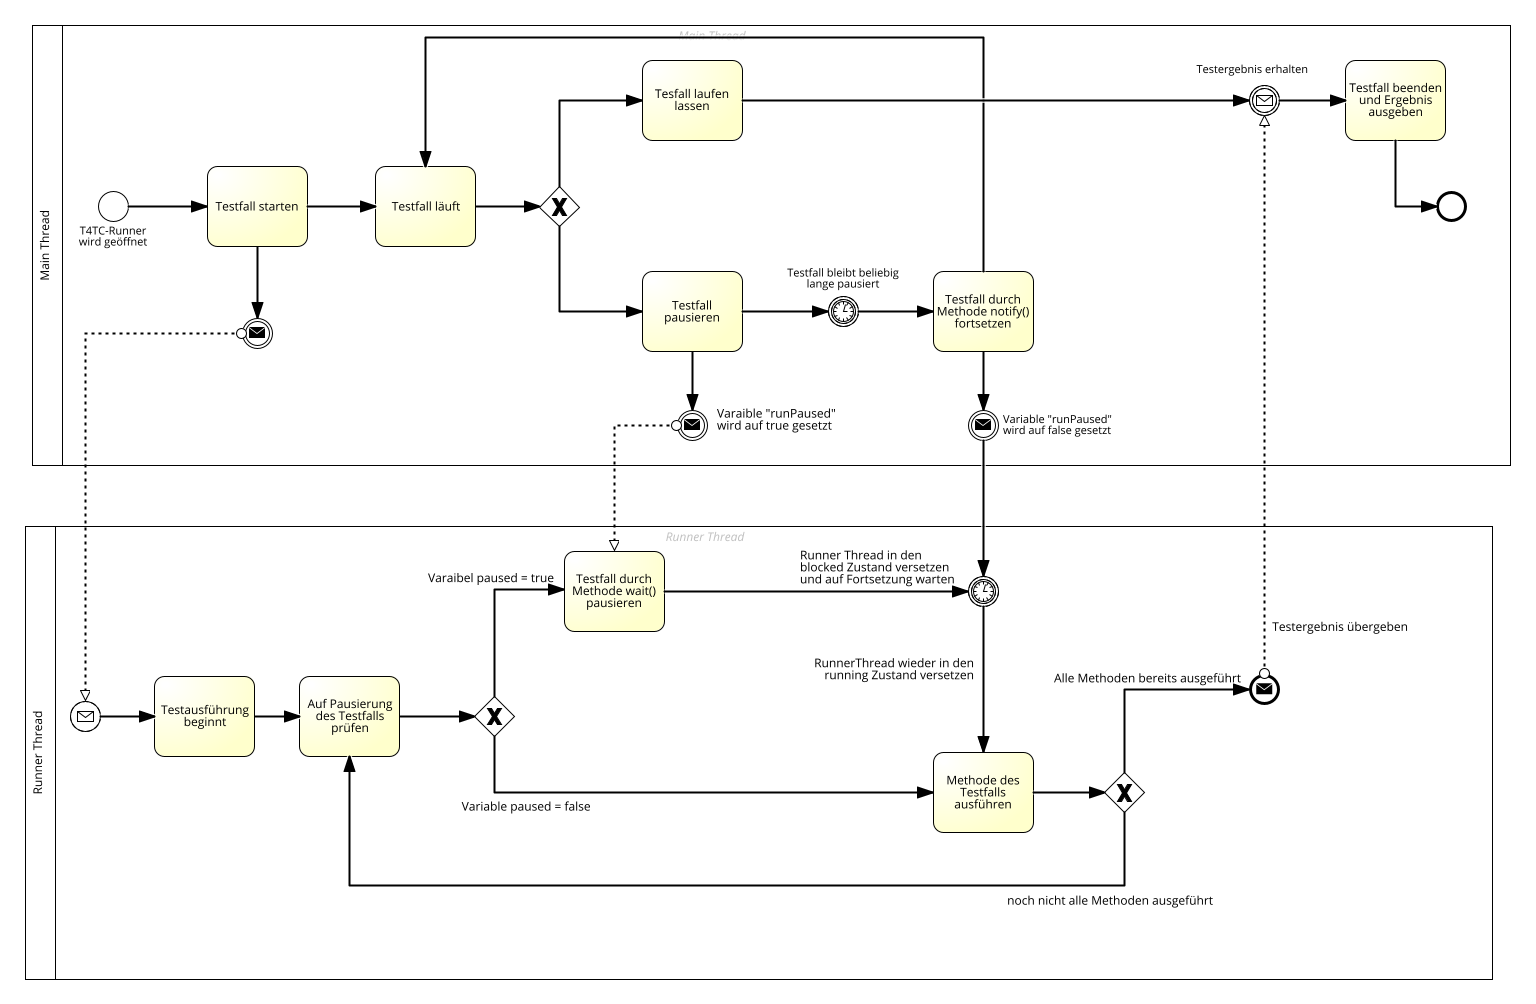
\includegraphics[scale=0.6, angle=90]{\imagedir/Pause-function (3).png}}
	\caption{vereinfachtes Prozessdiagramm der neuen Testausführung} \cite{Quelle: eigene Darsetllung}
	\label{BPMN}
\end{figure}
